% Hlavicka pro protokoly z fyzikalniho praktika.
% Verze pro: LaTeX
% Verze hlavicky: 22. 2. 2007
% Autor: Ustav fyziky kondenzovanych latek
% Ke stazeni: www.physics.muni.cz/ufkl/Vyuka/
% Licence: volne k pouziti, nejlepe k vcasnemu odevzdani protokolu z Vaseho mereni.

\documentclass[a4paper,11pt]{article}

% Kodovani (cestiny) v dokumentu: utf-8
%\usepackage[cp1250]{inputenc}	% Omezena stredoevropska kodova stranka, pouze MSW.
\usepackage[utf8]{inputenc}	% Doporucujeme pouzivat UTF-8 (unicode).
\usepackage[T1]{fontenc}
\usepackage{lmodern}

%%% Nemente:
\usepackage[margin=2cm]{geometry}
\newtoks\jmenopraktika \newtoks\jmeno \newtoks\datum
\newtoks\obor \newtoks\skupina \newtoks\rocnik \newtoks\semestr
\newtoks\cisloulohy \newtoks\jmenoulohy
\newtoks\tlak \newtoks\teplota \newtoks\vlhkost
\usepackage{amsmath}
\usepackage{mathtools}
\usepackage{graphicx}
\usepackage{multirow}

\usepackage{pgfplotstable} 
\usepackage{booktabs}

\graphicspath{ {./images/} }
%%% Nemente - konec.


%%%%%%%%%%% Doplnte pozadovane polozky:

\jmenopraktika={Physical laboratory 3}  % nahradte jmenem vaseho predmetu
\jmeno={Artem Gorodilov}            % nahradte jmenem mericiho
\datum={25. ~march 2024}        % nahradte datem mereni ulohy
\obor={Astrophysics}                     % nahradte zkratkou vami studovaneho oboru
\skupina={Mon 14:00}            % nahradte dobou vyuky vasi seminarni skupiny
\rocnik={II}                  % nahradte rocnikem, ve kterem studujete
\semestr={II}                 % nahradte semestrem, ve kterem studujete

\cisloulohy={G}               % nahradte cislem merene ulohy
\jmenoulohy={Bandwidth of prohibited energies} % nahradte jmenem merene ulohy

\tlak={979}                   % nahradte tlakem pri mereni (v hPa)
\teplota={21.4}               % nahradte teplotou pri mereni (ve stupnich Celsia)
\vlhkost={46}               % nahradte vlhkosti vzduchu pri mereni (v %)

%%%%%%%%%%% Konec pozadovanych polozek.


%%%%%%%%%%% Uzitecne balicky:
\usepackage[czech]{babel}
\usepackage{graphicx}
\usepackage{amsmath}
\usepackage{xspace}
\usepackage{url}
\usepackage{indentfirst}
\usepackage{listings}
\usepackage{subcaption}
\usepackage{caption}
\usepackage{tabularx}
\usepackage[labelformat=parens,labelsep=quad,skip=3pt]{caption}

%%%%%% Zamezeni parchantu:
\widowpenalty 10000 \clubpenalty 10000 \displaywidowpenalty 10000
%%%%%% Parametry pro moznost vsazeni vetsiho poctu obrazku na stranku
\setcounter{topnumber}{3}	  % max. pocet floatu nahore (specifikace t)
\setcounter{bottomnumber}{3}	  % max. pocet floatu dole (specifikace b)
\setcounter{totalnumber}{6}	  % max. pocet floatu na strance celkem
\renewcommand\topfraction{0.9}	  % max podil stranky pro floaty nahore
\renewcommand\bottomfraction{0.9} % max podil stranky pro floaty dole
\renewcommand\textfraction{0.1}	  % min podil stranky, ktery musi obsahovat text
\intextsep=8mm \textfloatsep=8mm  %\intextsep pro ulozeni [h] floatu a \textfloatsep pro [b] or [t]

% Tecky za cisly sekci:
\renewcommand{\thesection}{\arabic{section}.}
\renewcommand{\thesubsection}{\thesection\arabic{subsection}.}
% Jednopismenna mezera mezi cislem a nazvem kapitoly:
\makeatletter \def\@seccntformat#1{\csname the#1\endcsname\hspace{1ex}} \makeatother

\begin{document}

\thispagestyle{empty}

{
\begin{center}
\sf 
{\Large Institute of Physical Electronics Sci MU} \\
\bigskip
{\huge \bfseries PHYSICAL LABORATORY} \\
\bigskip
{\Large \the\jmenopraktika}
\end{center}

\bigskip

\sf
\noindent
\setlength{\arrayrulewidth}{1pt}
\begin{tabular*}{\textwidth}{@{\extracolsep{\fill}} l l}
\large {\bfseries Processed by:}  \the\jmeno & \large  {\bfseries Measured:} \the\datum\\[2mm]
\large  {\bfseries Field:} \the\obor  \hspace{40mm}  {\bfseries Group:} \the\skupina %
%{\bfseries Ročník:} \the\rocnik \hspace{5mm} {\bfseries Semestr:} \the\semestr  
&\large {\bfseries Validated:}\\
\\
\hline
\end{tabular*}
}

\bigskip

{
\sf
\noindent \begin{tabular}{p{3cm} p{0.6\textwidth}}
\Large  Problem №. {\bfseries \the\cisloulohy:} \par
\smallskip
% $T=\the\teplota$~$^\circ$C \par
% $p=\the\tlak$~hPa \par
% $\varphi=\the\vlhkost$~\%
&\Large \bfseries \the\jmenoulohy  \\[2mm]
\end{tabular}
}

\vskip10pt
    \begin{minipage}[t]{0.5\textwidth} 
        \section{Task}    
            Using the photoelectric effect, determine the strength of the forbidden energy band in silicon and germanium.
        \section{Theory}
            Solid materials are classified into conductors and insulators, with conductors further categorized into metals and semiconductors. The classification of a material into one of these groups is influenced by the band gap, which is the energy difference between the valence band and the conduction band. In metals, these bands overlap, allowing electrons to easily transition between levels, thereby enabling the material to conduct electricity. Semiconductors possess a relatively small band gap, which permits electrons to overcome this barrier through thermal activation. In contrast, insulators have a wide band gap, making thermal activation improbable.
            \par In this context, we will use a germanium and silicon PN junction as a semiconductor, which converts light signals into electrical signals by leveraging the internal photoelectric effect. During the internal photoelectric effect, valence electrons are excited into the conduction band. The absorption of radiation with different wavelengths occurs in layers of varying thickness. The variation in the intensity of the light signal within the material can be described by the equation:
            \begin{equation}
                I = I_0 R \cdot e^{-\alpha x}
            \end{equation}
            where $x$ represents the depth beneath the surface, $R$ is the material's reflectivity, $I_0$ is the original light intensity, and $\alpha$ is the absorption coefficient.
            \par This relationship demonstrates that photons with excessively long wavelengths lack the energy required for atom excitation.
    \end{minipage}
    \hspace{10pt}
    \begin{minipage}[t]{0.5\textwidth} 
            \vspace{10pt}   
            \par \centering
            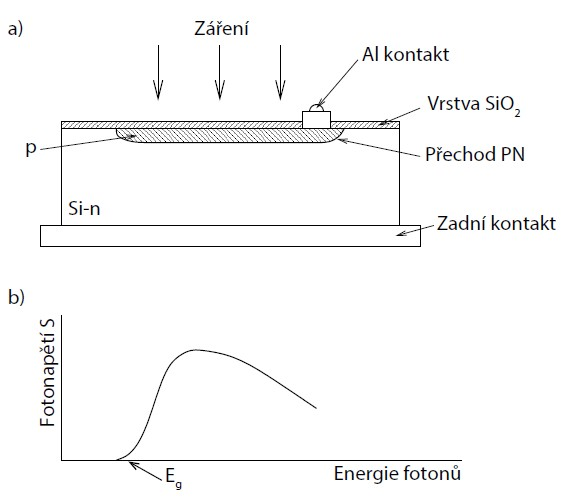
\includegraphics[scale=0.5]{scheme}
            \captionsetup{justification=centering, font=footnotesize}
            \captionof{figure}{(a) Schematic of the photodiode and (b) photovoltage dependence on photon energy.}
            \label{fig:scheme}
            \vspace{10pt}
            \raggedright   

            \par As the energy of the photons increases, excitation of atoms begins, generating a photovoltage at the photodiode. The photovoltage increases with decreasing wavelength, but beyond a certain point, it starts to decrease again. This decrease is due to the photons having too much energy, causing atom excitation to occur too deep below the surface of the photodiode and thus outside the PN junction area.
            \par By integrating aspects of physical theory, we've nuanced the explanation, focusing on the role of the band gap in determining electrical properties and detailing the function and significance of the PN junction in converting light to electrical signals through the photoelectric effect. 
            \par To find bandwidth of prohibited energies $E_g$ we need to find spectral dependence of photovoltage corresponded to one photon $S(\lambda)$. It could be represented as relation of photovoltage $U(\lambda)$ and number of detected photons $N(\lambda)$:
            \begin{equation}
                S(\lambda) = \frac{U(\lambda)}{N(\lambda)}
            \end{equation}
    \end{minipage}
\newpage
    \begin{minipage}[t]{0.5\textwidth} 
            From interchangeability of number of detected photons and so called relative intensity of photodetector signal $D(\lambda) \propto N(\lambda)$ we can write:
            \begin{equation}
                S(\lambda) \approx \frac{U(\lambda)}{D(\lambda)}
            \end{equation}
        \section{Měření}     
                For both silicon and germanium, we measured the spectral dependence of the photovoltage $U(\lambda)$ and the wavelength $\lambda$ of the light source. The photovoltage was measured using a analogue voltmeter, and the wavelength was determined using a monochorator. 
                \par We used equivalence of wavelength and energy to caltulate photon energy $E_f$. 
                \par Then, to determine $S(\lambda)$, we should firstly find $D(\lambda)$ corresponding to each wavelength $\lambda$ we where using. Do do it we used given data of spectral dependence of photodetector signal $D(\lambda)$, which is presented in table (5.1) and plot (2). We interpolated $D = f(\lambda)$ using \texttt{numpy.polyfit} with polinomial degree 3 and by this we found $D(\lambda)$ for each $\lambda$.

                \vspace{10pt}   
                \par \centering
                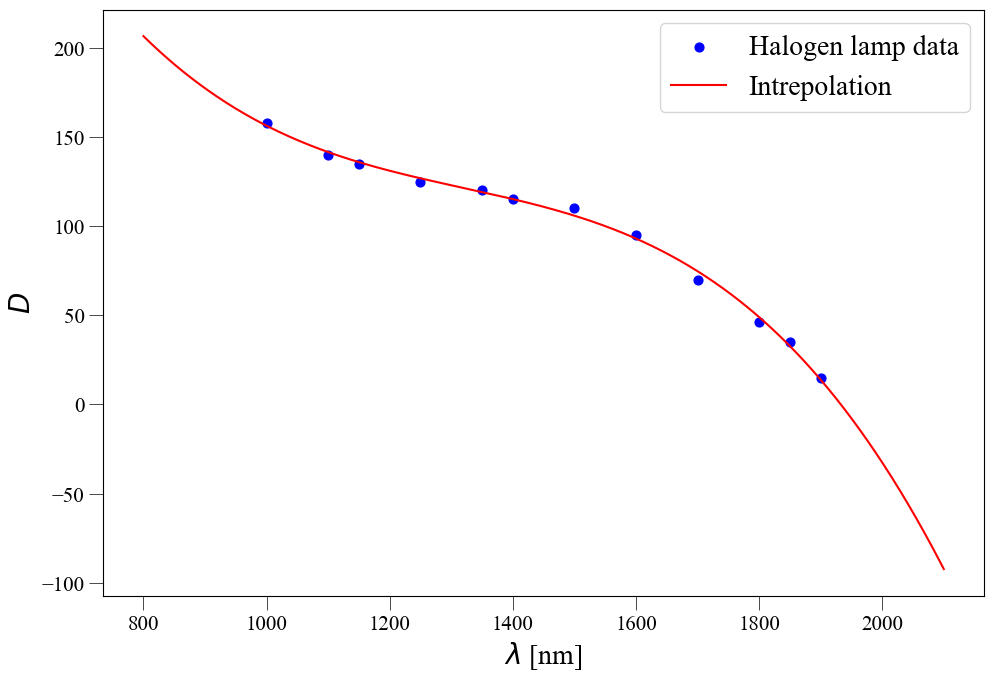
\includegraphics[scale=0.35]{int}
                \captionsetup{justification=centering, font=footnotesize}
                \captionof{figure}{Interpolation of spectral dependence of photodetector signal.}
                \label{fig:int}
                \vspace{10pt}
                \raggedright 

                \par Finally, we calculated $S(\lambda)$ using relation (3). 
                \par The results of the measurements for silicon and germanium are presented in tables (5.2) and (5.3) respectively.
                \par Then we plotted relation $S = f(E_f)$ for both materials. We fitted the data for selicon using polinomial fit with degree 5 and for germanium using polinomial fit with degree 4. Knowing, that energy of prohibited band could be found, by dividing relation $S = f(E_f)$ by 2, and looking on corresponding energy at the left side of a plot. The results are presented in figures (3) and (4) respectively.

                
    \end{minipage}
    \hspace{10pt}
    \begin{minipage}[t]{0.5\textwidth} 
                \vspace{0pt}   
                \par \centering
                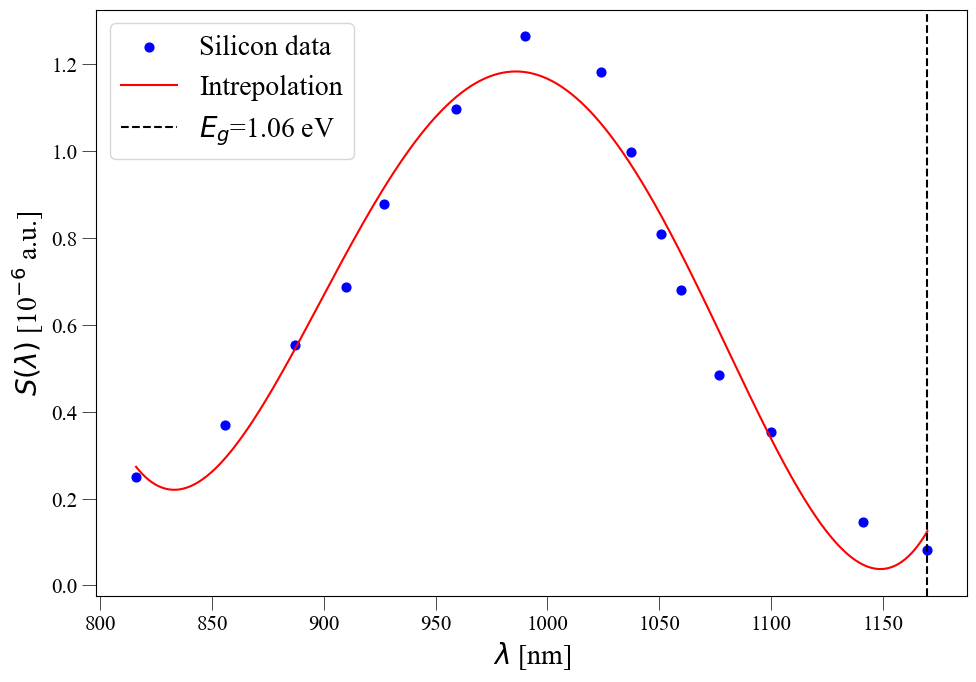
\includegraphics[scale=0.35]{sil}
                \captionsetup{justification=centering, font=footnotesize}
                \captionof{figure}{Spectral dependence of photovoltage for silicon.}
                \label{fig:sil}
                \raggedright  

                \vspace{10pt}   
                \par \centering
                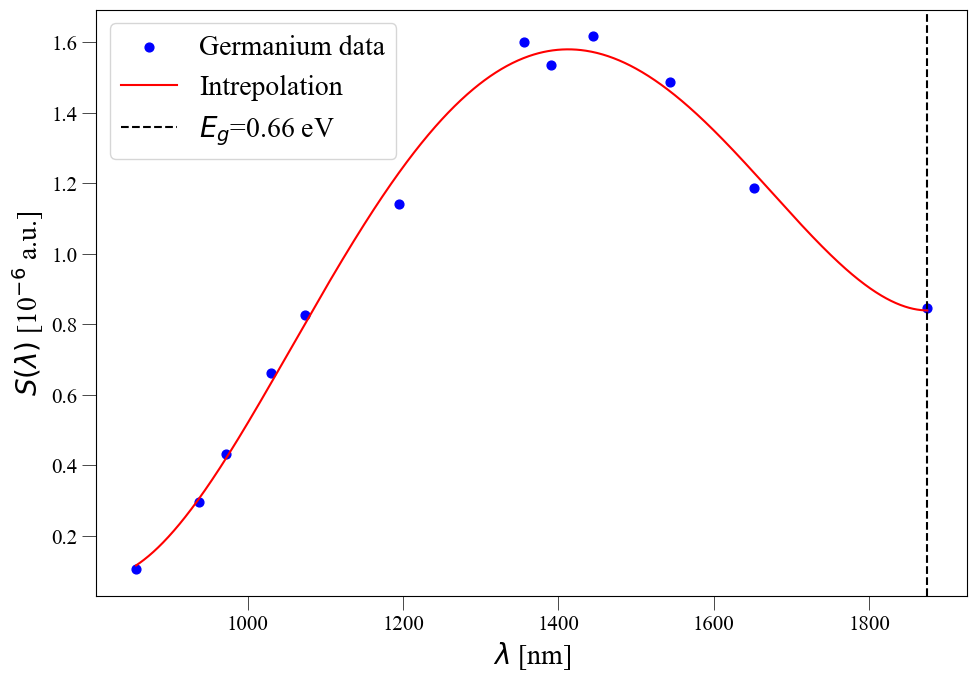
\includegraphics[scale=0.35]{ger}
                \captionsetup{justification=centering, font=footnotesize}
                \captionof{figure}{Spectral dependence of photovoltage for germanium.}
                \label{fig:sil}
                \vspace{10pt}
                \raggedright 

                \par From the results of the measurements, we can see that the energy of the forbidden band are: 
                \begin{center}
                    $E_{g, Si} = 1.06(1)$ eV and $E_{g, Ge} = 0.66(1)$ eV.
                \end{center}

                \par The Uncertinties library for Python\cite{uncertainties} was used to calculate the variables and their uncertainties. The errors were augmented with the Student's coefficient (2-Tail Confidence Level) with respect to the degrees of freedom for each value, for a confidence interval of 68.27\%.
        
        \section{Conclution} 
                Obtained values of the forbidden energy band for silicon and germanium $E_{g, Si} = 1.06(1)$ eV and $E_{g, Ge} = 0.66(1)$ eV, are in good agreement with the literature values of $E_{g, Si} = 1.13(2)$ eV and $E_{g, Ge} = 0.65(1)$ eV \cite{collings}. 
                \par The difference could be explained by the fact that the measurements were conducted by not so precice in the sence of reading wavelenth and photovoltage, because of some fluctuations of the signal and changing scale of monochorator.

    \end{minipage}
\newpage
                \begin{thebibliography}{9}
                    \bibitem{uncertainties}
                        Uncertainties, Available online: \url{https://pypi.org/project/uncertainties}
                    \bibitem{collings}
                        Collings, P. (1980). Simple Measurement of the Band Gap in Silicon and Germanium.. American Journal of Physics, 48, 197-199. \url{https://doi.org/10.1119/1.12172}
                \end{thebibliography} 

    \begin{center}
        \section{Appendix}
            \begin{center}
                \subsection{Table of spectral emission of a halogen lamp.} 
                    \pgfplotstabletypeset[
                        col sep=comma, % Defines the separator, comma for CSV
                        string type, % Treats columns as strings (not math mode)
                        every head row/.style={before row=\toprule,after row=\midrule},
                        every last row/.style={after row=\bottomrule},
                        columns/lam/.style={column name=$\lambda$ [nm]},
                        columns/D/.style={column name=D(\lambda)}
                    ]{data/d_lam.csv} 
            \end{center}
            \begin{center}
                \subsection{Table of spectral dependence of photovoltage for silicon.}
                    \pgfplotstabletypeset[
                        col sep=comma, % Defines the separator, comma for CSV
                        string type, % Treats columns as strings (not math mode)
                        every head row/.style={before row=\toprule,after row=\midrule},
                        every last row/.style={after row=\bottomrule},
                        columns/U/.style={column name=U [mV]},
                        columns/lam/.style={column name=$\lambda$ [nm]},
                        columns/E/.style={column name=$E_f$ [eV]},
                        columns/D/.style={column name=D(\lambda)},
                        columns/S/.style={column name=S(\lambda) [10$^{-6}$ a.u.]},
                    ]{data/sil.csv} 
            \end{center}
            \begin{center}
                \subsection{Table of spectral dependence of photovoltage for germanium.}
                    \pgfplotstabletypeset[
                        col sep=comma, % Defines the separator, comma for CSV
                        string type, % Treats columns as strings (not math mode)
                        every head row/.style={before row=\toprule,after row=\midrule},
                        every last row/.style={after row=\bottomrule},
                        columns/U/.style={column name=U [mV]},
                        columns/lam/.style={column name=$\lambda$ [nm]},
                        columns/E/.style={column name=$E_f$ [eV]},
                        columns/D/.style={column name=D(\lambda)},
                        columns/S/.style={column name=S(\lambda) [10$^{-6}$ a.u.]},
                    ]{data/ger.csv}
            \end{center}
\end{document}